\documentclass[compress]{beamer}

\usepackage[brazil,portuguese]{babel}
\usepackage[utf8]{inputenc}
%\usepackage{caption}
%\usepackage{subcaption}
\usepackage{ragged2e}
\usepackage{graphicx}
\usepackage{tikz}
\usetikzlibrary{positioning}
\usetikzlibrary{decorations.pathreplacing}
\usetikzlibrary{decorations.pathmorphing}
\usetikzlibrary[patterns]
\usetikzlibrary{calc}
\usepackage{pgfplots}
\pgfplotsset{compat=newest}
\usepackage{amsfonts}
\usepackage{amssymb}
\usepackage{amsmath}
\usepackage{MnSymbol}
\usepackage[Algoritmo]{algorithm}
\usepackage[noend]{algorithmic}
\setbeamertemplate{bibliography entry title}{}
\setbeamertemplate{bibliography entry location}{}
\setbeamertemplate{bibliography entry note}{}

\newcounter{saveenumi}

\newcommand{\seti}{\setcounter{saveenumi}{\value{enumi}}}
\newcommand{\conti}{\setcounter{enumi}{\value{saveenumi}}}
\newtheorem{teorema}[theorem]{\scshape Teorema}
\newtheorem{proposicao}[theorem]{\scshape Proposição}
\newtheorem{corolario}[theorem]{\scshape Corolário}
\newtheorem{lema}[theorem]{\scshape Lema}
\newtheorem{definicao}[theorem]{\scshape Definição}
\newtheorem{conjectura}[theorem]{\scshape Conjectura}
\newtheorem{escolio}[theorem]{\scshape Escólio}
\newtheorem{exemplo}[theorem]{\scshape Exemplo}
\newtheorem{exemplos}[theorem]{\scshape Exemplos}
\newtheorem{propriedade}[theorem]{\scshape Propriedade}

\renewcommand{\u}{{\bf u}}
\renewcommand{\v}{{\bf v}}
\renewcommand{\sin}{\operatorname{sen}}
\renewcommand{\tan}{\operatorname{tg}}
\providecommand{\cas}{\operatorname{cas}}
\providecommand{\mdc}{\mathrm{mdc}}
\providecommand{\f}{{\bf f}}

\newcommand{\ie}{\textit{i.e.}}
\newcommand{\eg}{\textit{e.g.}}
\renewcommand\Re{\operatorname{Re}}
\renewcommand\Im{\operatorname{Im}}

\providecommand{\x}{{\bf x}}
\providecommand{\y}{{\bf y}}
\providecommand{\w}{{\bf w}}
\providecommand{\f}{{\bf f}}
\providecommand{\q}{{\bf q}}
\providecommand{\bfa}{{\bf a}}
\providecommand{\bfb}{{\bf b}}
\providecommand{\bfc}{{\bf c}}
\providecommand{\bfd}{{\bf d}}
\providecommand{\bfe}{{\bf e}}
\providecommand{\bfs}{{\bf s}}
\providecommand{\bfz}{{\bf z}}
\providecommand{\zero}{{\bf 0}}
\providecommand{\spn}{\mathrm{span}}
\providecommand{\posto}{\mathrm{posto}}
\providecommand{\nul}{\mathrm{nul}}
\providecommand{\proj}{\mathrm{proj}}
\providecommand{\tr}{\mathrm{tr}}
\providecommand{\sgn}{\mathrm{sgn}}
\providecommand{\cov}{\mathrm{cov}}
\providecommand{\dilation}{\mathcal{D}}
\providecommand{\erosion}{\mathcal{E}}
\providecommand{\open}{\mathcal{O}}
\providecommand{\close}{\mathcal{C}}

\newcommand*{\Bhat}{\skew{3}{\hat}{B}}

\mode<presentation>
{
  \setbeamertemplate{background canvas}[vertical shading][bottom=white!10,top=blue!10]
%  \usetheme{Berkeley}
%  \usetheme{CambridgeUS}
%  \usetheme{Madrid}
  \usetheme{Warsaw}
  \usefonttheme[onlysmall]{structurebold}  
  \setbeamertemplate{headline}{}  
% \setbeamercovered{invisible} % default
  \setbeamercovered{transparent, again covered={\opaqueness{25}} } % =15%
% \setbeamercovered{transparent=50}
% \setbeamercovered{dynamic}
% \setbeamercovered{again covered={\opaqueness<1->{25}}}
}

\usepackage{ifthen}
\makeatletter
\newcommand{\includecoveredgraphics}[2][]{
    \ifthenelse{\the\beamer@coveringdepth=1}{
        \tikz
            \node[inner sep=0pt,outer sep=0pt,opacity=0.15]
                {\includegraphics[#1]{#2}};
    }{
        \tikz
            \node[inner sep=0pt,outer sep=0pt]
                {\includegraphics[#1]{#2}};%
    }
} 
%\makeatother

%%% CAPA %%%
\title{Usando criptografia de forma prática e descomplicada}
\author{Marcos Azevedo aka psylinux}
\date{BSidesSP - Edição 0xF - Maio 2018 }


%%% APRESENTAÇÃO %%%
\begin{document}
\frame{\titlepage}

%%% SUMÁRIO %%%
%\section{Sumário}
%\frame{\tableofcontents}
%\section{}

\begin{frame}
\frametitle{Sumário}
	\begin{enumerate}
		\item<+->{Apresentação Pessoal}
		\item<+->{Qual a relevância desse tema?}
		\item<+->{História da Criptografia}
		\begin{enumerate}
			\item<+->{Cifra de César}
		\end{enumerate}
		\item<+->{Introdução à criptografia}
		\begin{enumerate}
			\item<+->{Definições e terminologias}
			\item<+->{Visão geral e funcionamento básico}
		\end{enumerate}
		\item<+->{Alguns tipos de criptografia}
		\begin{enumerate}
			\item<+->{Criptografia Simétrica}
			\item<+->{Criptografia Assimétrica}
			\item<+->{Assinatura Digital}
		\end{enumerate}
		\item<+->{Ferramentas para usar no dia-a-dia (Linux e Windows)}
		\begin{enumerate}
			\item<+->{GPG e PGP}
			\item<+->{Assinatura de Arquivo}
			\item<+->{Criptografia de Arquivos}
			\item<+->{Assinatura de E-mail}
			\item<+->{Criptografia em E-mail}
			\item<+->{Chave GPG para Login em SSH}
		\end{enumerate}
		\item<+->{Considerações finais}
	\end{enumerate}
\end{frame}

%\begin{frame}
%	{\tableofcontents}
%\end{frame}

%%% SLIDE %%%
\begin{frame}
\frametitle{Apresentação Pessoal}
	\justifying
		Marcos Azevedo - Consultor de Segurança na Cipher. Possui mais de 15 anos de experiência em Segurança da Informação, onde os últimos quatro anos foram dedicados a hardening de servidores, correção de problemas de segurança, análise forense, pentesting e segurança ofensiva. Ele tem um bom conhecimento de sistemas operacionais, arquitetura de computadores, compiladores e montadores para Intel x86, linguagem C, Python, PowerShell Scripts e Shell Scripts. Possui um sólido conhecimento de protocolos TCP/IP e experiência em infraestrutura de rede (Cisco Routers and Switches). Sua curva de aprendizado é muito rápida graças aos seus conhecimentos sólidos dos princípios da computação, além da motivação por desafios. Marcos já palestrou em conferências tais como: H2HC, FLISOL, FGSL e outros.
\end{frame}

%%% SLIDE %%%
\begin{frame}
\frametitle{Apresentação Pessoal}
	\begin{figure}[h]
		\caption{Goiânia, Goiás}
		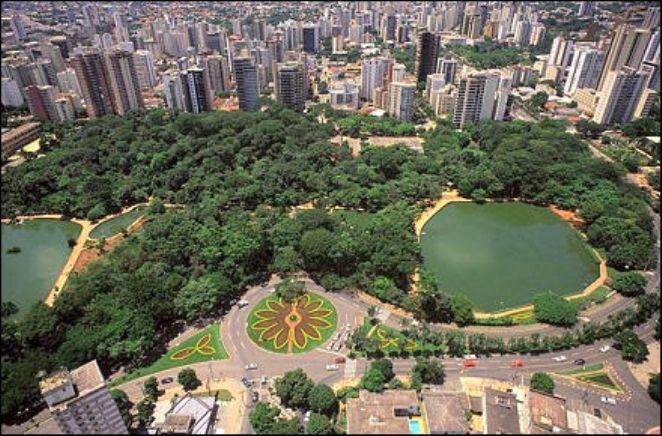
\includegraphics[width=\textwidth]{pics/goiania}
	\end{figure}
\end{frame}

%%% SLIDE %%%
\begin{frame}
\frametitle{Goianês, Codificação ou Criptografia?}
\framesubtitle{Introdução}
	\begin{itemize}
		\justifying
		\item<+->{\textbf{Dinheiro pra sapecar porco}: Muito dinheiro.}
		\item<+->{\textbf{Custoso (a)}: Difícil, pessoa sapeca.}
		\item<+->{\textbf{Demais da conta}: Muito, muito mesmo.}
		\item<+->{\textbf{Encabulado}: Impressionado.}
		\item<+->{\textbf{Pizêro}: Bagunça.}
		\item<+->{\textbf{Pulá o corguim}: Passar dos limites.}
		\item<+->{\textbf{Apiar}: Descer.}
		\item<+->{\textbf{Rudeia/Rudiá}: Dar a volta.}
	\end{itemize}
\end{frame}

%%% SLIDE %%%
\begin{frame}
\frametitle{Antes de Começar o Assunto}
\framesubtitle{Criptografia vs Codificação}
\centering 
\textbf{\Huge Criptografia vs Codificação}\\
{\Huge Tem diferença?}
\end{frame}

%%% SLIDE %%%
\begin{frame}
\frametitle{Criptografia vs Codificação}
\framesubtitle{Codificação}
	\begin{enumerate}
		\justifying
		\item<+->{\textbf{Objetivo da Codificação:} transformar os dados para que ele possa ser adequadamente utilizado por um diferente tipo de sistema, por exemplo, caracteres especiais de uma página web. Não serve para manter em segredo as informações, mas sim garantir que o sistema interprete de outra forma os dados contidos na mensagem.}
		\item<+->{\textbf{Exemplos:} ASCII, Unicode, URL Encoding, Base64.}
	\end{enumerate}
\end{frame}

%%% SLIDE %%%
\begin{frame}
\frametitle{Criptografia vs Codificação}
\framesubtitle{Criptografia}
	\begin{enumerate}
		\justifying
		\item<+->{\textbf{Objetivo da Criptografia:} transformar os dados, afim de manter uma “mensagem” em segredo e garantir que os dados sejam inteligíveis apenas para o destinatário com a chave para reverter a criptografia.}
	\end{enumerate}
\end{frame}

%%% SLIDE %%%
\begin{frame}
\frametitle{Visão Geral}
\framesubtitle{O que é Criptografia?}
	\begin{figure}[h]
		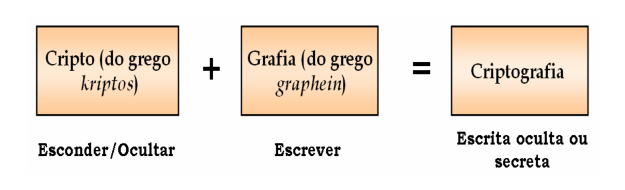
\includegraphics[width=\textwidth]{pics/cripto_1}
	\end{figure}
\end{frame}

%%% SLIDE %%%
\begin{frame}
\frametitle{Qual a relevância desse tema?}
	\centering
	\textbf{\LARGE "Criptografia"}\\
	\textbf{\LARGE Qual a relevância desse tema?}
\end{frame}

%%% SLIDE %%%
\begin{frame}
	\frametitle{Qual a relevância desse tema?}
	\framesubtitle{Por que usamos criptografia?}
	\centering
		Quando queremos que apenas o \textbf{EMISSOR} e o \textbf{DESTINATÁRIO} compreendam o conteúdo da mensagem.
\end{frame}

%%% SLIDE %%%		
\begin{frame}
\frametitle{Qual a relevância desse tema?}
\framesubtitle{Quando usamos criptografia?}
	\begin{itemize}
		\justifying
		\item<+->{\textbf{"Em trânsito"}, neste contexto, é quando você envia informações através da Internet, por e-mail ou quando precisa armazená-la em outro lugar que não seja o seu próprio dispositivo.}
		\item<+->{\textbf{"Em repouso"}, quando estão armazenados em seu dispositivo, que pode ser parte integrada como um disco rígido, ou em um meio removível, como uma unidade USB.}
	\end{itemize}
\end{frame}

%%% SLIDE %%%		
\begin{frame}
\frametitle{Tipos de Criptografia}
\begin{enumerate}
	\justifying
	\item<+->{\textbf{Criptografia Clássica:} Sustenta-se em leis matemáticas. Já era utilizado nos hieróglifos de monumentos do Antigo Egito (cerca de 4500 anos atrás).}
	\item<+->{\textbf{Criptografia Moderna:} Utiliza basicamente os mesmos princípios da Criptografia Clássica, mas faz uso de computadores para processar os dados. Consideramos seu inicio em 1949 com Matemático Americano Claude Shannon.}
	\item<+->{\textbf{Criptografia Quântica:} Utiliza-se de elementos físicos, tal com fótons, para gerar chaves quânticas \emph{inquebráveis}.}
\end{enumerate}
\end{frame}

%%% SLIDE %%%		
\begin{frame}
\frametitle{Criptografia Moderna}
\framesubtitle{Algoritmos Criptográficos}
\begin{enumerate}
	\justifying
	\item<+->{\textbf{Algoritmo de transposição:} rearranja a ordem dos caracteres de uma mensagem. Um exemplo simples é a transformação de \textbf{“muito obrigado”} em \textbf{“omtui oobdraig”}. Esta categoria de algoritmo criptográfico é composta por uma função bijetora	para efetuar encriptações e sua	inversa faz a mensagem voltar à forma original;}
	\item<+->{\textbf{Algoritmo de substituição:} substitui caracteres ou grupos de caracteres por outros caracteres ou grupos de caracteres. Um exemplo simples: \textbf{“muito obrigado”} é transformado em \textbf{“nvjup pcsjhbep”}, substituindo cada letra pela próxima na sequência alfabética.}
\end{enumerate}
\end{frame}

%%% SLIDE %%%
\begin{frame}
\frametitle{Alguns algoritmos da Criptografia Moderna}
	\begin{enumerate}
		\justifying
		\item \textbf{Algoritmo de Euclides:} Ele é um elemento-chave dos algoritmos RSA (Criptografia de Chaves Assimétricas).
		\item \textbf{Transformada de Fourier:} Utilizada em esteganografia.
		\item \textbf{Algoritmos de Aritmética Modular:} Também conhecida como aritmética do relógio, aplicado a números inteiros. Utilizada em Criptografia de Chave Simétrica, CPF, Código de Barras.
	\end{enumerate}
\end{frame}

%%% SLIDE %%%
\begin{frame}
\frametitle{Entendendo o Algoritmo de Euclides}
\begin{figure}[h]
	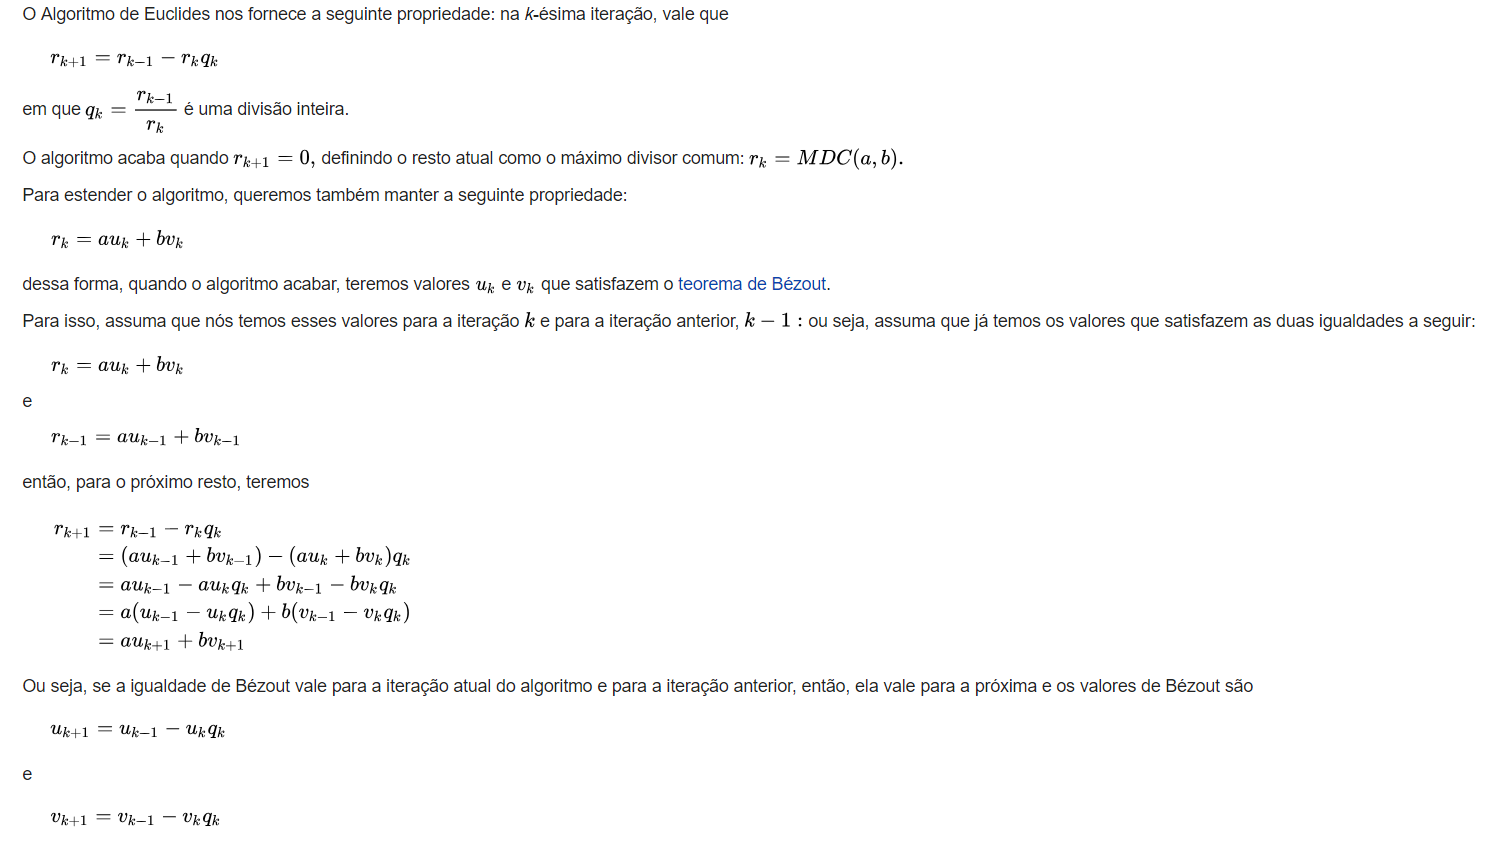
\includegraphics[width=\textwidth]{pics/euclides_1}
\end{figure}
\end{frame}

%%% SLIDE %%%
\begin{frame}
\frametitle{Criptografia Clássica}
\framesubtitle{Algoritmo de Transposição}
\centering
\textbf{{\LARGE BRINCADEIRA GENTE!}}
\end{frame}

%%% SLIDE %%%
\begin{frame}
\frametitle{Criptografia Clássica}
\framesubtitle{Algoritmo de Transposição}
\centering
Mensagem: \textbf{CRIPTOGRAFIA NA BSIDES SAO PAULO 2018}
\end{frame}

%%% SLIDE %%%		
\begin{frame}
\frametitle{Criptografia Clássica}
\framesubtitle{Algoritmo de Transposição}
	\begin{figure}[h]
		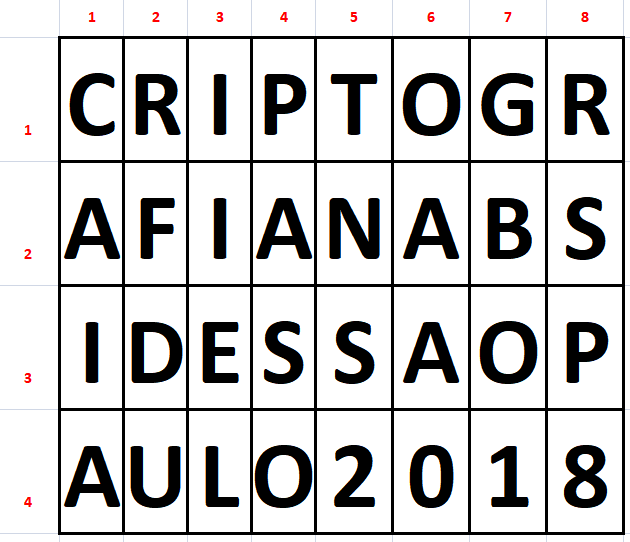
\includegraphics[width=\textwidth,height=7cm]{pics/tab_trans_1}
	\end{figure}
\end{frame}

%%% SLIDE %%%
\begin{frame}
\frametitle{Criptografia Clássica}
\framesubtitle{Algoritmo de Transposição}
\centering
Chave criptográfica: \textbf{24176835}
\end{frame}

%%% SLIDE %%%		
\begin{frame}
\frametitle{Criptografia Clássica}
\framesubtitle{Algoritmo de Transposição}
\begin{figure}[h]
	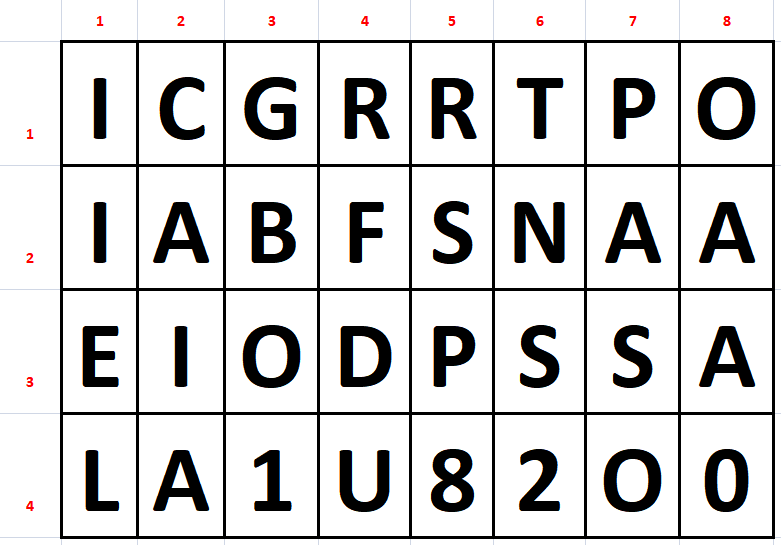
\includegraphics[width=\textwidth,height=7cm]{pics/tab_trans_2}
\end{figure}
\end{frame}

%%% SLIDE %%%		
\begin{frame}
\frametitle{Criptografia Clássica}
\framesubtitle{Algoritmo de Substituição}
\justifying
3M UM D14 D3 VER40, 3S7AVA N4 PR4I4,O853RV4NDO DU4S CR14NÇ4S 8B1NC4ND0 N4 4REI4. EL45 TR4B4LH4V4M MUI7O C0N57R1ND0 UM C4ATEL0 D3 AR3I4, C0M 70RR35, P4554R3L4S 3 P4554G3N5 1N7ERN4S. QU4ND0 ES74V4M QU4S3 T3RM1N4ND0, V310 UM4 0ND4 3 3S7RU1U 7UDO, R3DU21NDO 0 C4S7EL0 4 UM MON73 D3 4REI4 3 3SPUM4. 4CH31 QU3 D3P01S D3 74N70 35FORÇ0 3 CU1D4D0, 45 CR1ANC4S C4IR4M N0 CH0R0,
CORR3R4M P3L4 PR41A, FUG1ND0 DA 4GU4, R1NDO D3 M405 D4D4S 3 C0M3C4R4M 4 C0NS7RU1R 0UTR0 C4573LO. 
\end{frame}


%%% SLIDE %%%		
\begin{frame}
\frametitle{Algumas Aplicações da Criptografia Atualmente}
		\begin{enumerate}
			\item{Sigilo em banco de dados;}
			\item{Censos;}
			\item{Investigações governamentais;}
			\item{Dossiês de pessoas sob investigação;}
			\item{Dados hospitalares;}
			\item{Informações de crédito pessoal;}
			\item{Decisões estratégicas empresariais;}
			\item{Sigilo em comunicação de dados;}
			\item{Comandos militares;}
			\item{Mensagens diplomáticas;}
			\item{Operações bancárias;}
			\item{Comércio eletrônico;}
			\item{Transações por troca de documentos eletrônicos (EDI);}
			\item{Estudo de idiomas desconhecidos;}
			\item{Recuperação de documentos arqueológicos, hieróglifos;}
			\item{E até tentativas de comunicações extraterrestres.}
		\end{enumerate}
\end{frame}

%%% SLIDE %%%		
\begin{frame}
\frametitle{Introdução à Criptografia}
\framesubtitle{Definições e terminologias | Criptologia}
\justifying
	\textbf{Criptologia:} disciplina que reúne os conhecimentos e as técnicas necessários à criptoanálise ('solução de criptogramas') e à criptografia ('modificação codificada').
\end{frame}

%%% SLIDE %%%		
\begin{frame}
\frametitle{Introdução à Criptografia}
\framesubtitle{Definições e terminologias | Texto Claro}
\justifying
\textbf{Texto Claro:} Texto original, não cifrado.
\end{frame}

%%% SLIDE %%%		
\begin{frame}
\frametitle{Introdução à Criptografia}
\framesubtitle{Definições e terminologias | Texto Cifrado}
\justifying
\textbf{Texto Cifrado:} Texto ilegível, não compreensível.
\end{frame}

%%% SLIDE %%%		
\begin{frame}
\frametitle{Introdução à Criptografia}
\framesubtitle{Definições e terminologias | Simetria}
\justifying
	\textbf{Simetria:} conformidade, em medida, forma e posição relativa, entre as partes dispostas em cada lado de uma linha divisória, um plano médio, um centro ou um eixo.
\end{frame}

%%% SLIDE %%%		
\begin{frame}
\frametitle{Introdução à Criptografia}
\framesubtitle{Definições e terminologias | Simetria}
\begin{figure}[h]
	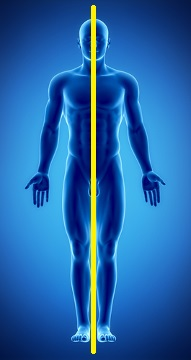
\includegraphics[height=7cm]{pics/simetria-bilateral}
\end{figure}
\end{frame}

%%% SLIDE %%%		
\begin{frame}
\frametitle{Introdução à Criptografia}
\framesubtitle{Definições e terminologias | Assimetria}
\justifying
	\textbf{Assimetria:} 1. ausência de simetria. 2. grande diferença; disparidade, discrepância. 
\end{frame}

%%% SLIDE %%%		
\begin{frame}
\frametitle{Introdução à Criptografia}
\framesubtitle{Definições e terminologias | Assimetria}
\begin{figure}[h]
	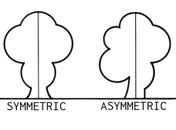
\includegraphics[height=7cm]{pics/assimetria}
\end{figure}
\end{frame}


%%% SLIDE %%%		
\begin{frame}
\frametitle{Introdução à Criptografia}
\framesubtitle{Definições e terminologias | Encriptar/Cifrar}
\justifying
	\textbf{Encriptar/Cifrar:} 1. reproduzir (mensagem) em código não conhecido, tornando-a, desse modo, intencionalmente ininteligível para os que não têm acesso às suas convenções. 2. inf codificar (informação) de modo que somente destinatários autorizados possam ter acesso a ela; encriptar.
\end{frame}

%%% SLIDE %%%		
\begin{frame}
\frametitle{Introdução à Criptografia}
\framesubtitle{Definições e terminologias | Decriptar/Decifrar}
\justifying
	\textbf{Decriptar/Decifrar:} traduzir ou decifrar mensagens ou códigos cifrados ou criptografados
\end{frame}

%%% SLIDE %%%		
\begin{frame}
\frametitle{Introdução à Criptografia}
\framesubtitle{Definições e terminologias | Bit}
\justifying
	\textbf{Bit:} menor parcela de informação processada por um computador. Algarismo do sistema binário que somente pode assumir as formas 0 ou 1
\end{frame}

%%% SLIDE %%%		
\begin{frame}
\frametitle{Introdução à Criptografia}
\framesubtitle{Definições e terminologias | Algoritmo}
\justifying
	\textbf{Algoritmo:} 1. mat sequência finita de regras, raciocínios ou operações que, aplicada a um número finito de dados, permite solucionar classes semelhantes de problemas. 2. inf conjunto das regras e procedimentos lógicos perfeitamente definidos que levam à solução de um problema em um número finito de etapas.
\end{frame}

%%% SLIDE %%%		
\begin{frame}
\frametitle{Introdução à Criptografia}
\framesubtitle{Funções Hash}
\justifying
O processo é unidirecional e impossibilita descobrir o conteúdo original a partir do Hash. O valor de conferência ("Soma de verificação") muda se um único bit for alterado, acrescentado ou retirado da mensagem.
	\begin{itemize}
		\justifying
		\item<+->{\textbf{Objetivo das funções de HASH:} Sua única finalidade é fazer um "resumo" representado em base hexadecimal que permite  visualização em letras (A a F) e números (0 a 9). O conceito teórico diz que "hash" é a transformação de uma grande quantidade de dados em uma pequena quantidade de informações".}
		\item<+->{\textbf{Exemplos:} MD4, MD5, SHA-1, SHA-512.}
	\end{itemize}	
\end{frame}

%%% SLIDE %%%
\begin{frame}
\frametitle{O Princípio de Kerckhoff}
	\center
	O Princípio de Kerckhoff é um princípio fundamental na criptografia moderna: \\
	\textbf{"Um sistema de criptografia deve ser seguro mesmo se o adversário conhecer todos os detalhes do sistema, com exceção da chave secreta."}
\end{frame}

%%% SLIDE %%%
\begin{frame}
\frametitle{Algoritmos Cifradores}
\justifying
	\begin{enumerate}
		\item<+->{\textbf{Cifradores de blocos:} divide a mensagem em blocos de tamanho fixo (ex: 256 bits). Por exemplo, DES, AES, 3DES}
		\item<+->{\textbf{Cifradores de fluxo:} cifra cada digito do texto plano por vez. Por exemplo, o RC4}
	\end{enumerate}
\end{frame}


%%% SLIDE %%%
\begin{frame}
\frametitle{Alguns tipos de Chaves Criptográficas}
		\begin{enumerate}
			\item<+->{Criptografia de Chave Simétrica}
			\item<+->{Criptografia de Chaves Assimétricas}
			\item<+->{Esquemas Híbridos}
		\end{enumerate}
\end{frame}

%%% SLIDE %%%
\begin{frame}
\frametitle{Criptografia de Chave Simétrica}
\begin{enumerate}
	\item<+->{Todos os esquemas de encriptação desde a antiguidade até 1976 eram simétricos.}
	\item<+->{Também conhecido como: criptografia de chave única ou criptografia de chave secreta.}
	\item<+->{A chave precisa ser transmitida através de um canal seguro.}
	\item<+->{Transmissão Wireless com protocolo \textbf{WPA (Wi-Fi Protected Access)} \footnote{Em 16 de Outubro de 2017, foi divulgado uma vulnerabilidade crítica (KRACK) que afeta milhões de dispositivos.} utilizam esse modelo criptográfico.}
\end{enumerate}
\end{frame}

%%% SLIDE %%%
\begin{frame}
\frametitle{Criptografia de Chave Simétrica}
\framesubtitle{Criptografando}
	\begin{figure}[h]
		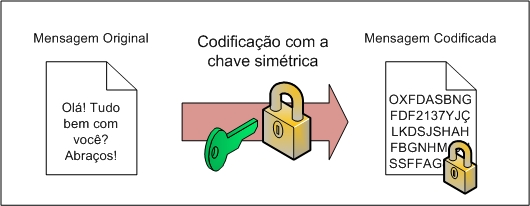
\includegraphics[width=\textwidth]{pics/chave_simetrica_1}
		\caption{Criptografando com chave simétricas\footnote{Imagem extraída de: https://www.gta.ufrj.br}}		
	\end{figure}
\end{frame}

%%% SLIDE %%%
\begin{frame}
\frametitle{Criptografia de Chave Simétrica}
\framesubtitle{Descriptografando}
\begin{figure}[h]
	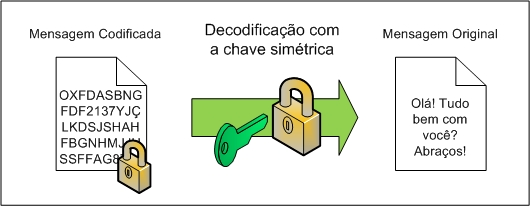
\includegraphics[width=\textwidth]{pics/chave_simetrica_2}
	\caption{Descriptografando com chaves simétricas\footnote{Imagem extraída de: https://www.gta.ufrj.br}}		
\end{figure}
\end{frame}

%%% SLIDE %%%
\begin{frame}
\frametitle{Criptografia de Chave Simétrica}
\justifying Exemplos de algoritmos simétricos populares:
	\begin{enumerate}
	\item AES
	\item Twofish
	\item Serpent
	\item Blowfish
	\item CAST5
	\item RC4
	\item 3DES (baseado no DES)
	\item IDEA
	\end{enumerate}
\end{frame}

%%% SLIDE %%%
\begin{frame}
\frametitle{Criptografia de Chaves Simétricas}
\framesubtitle{Problemas com as Chaves Simétricas}
	\begin{itemize}
		\item<+->{Como distribuir as chaves de maneira segura?}
		\item<+->{Como verificar se a mensagem não foi modificada?}
		\item<+->{Como ter certeza que a mensagem foi realmente enviada por quem diz ter enviado?}
	\end{itemize}
\end{frame}

%%% SLIDE %%%
\begin{frame}
\frametitle{Criptografia de Chaves Assimétricas}
\framesubtitle{Visão Geral}
\begin{enumerate}
	\item<+->{Em 1976, Diffie, Hellman e Merkle propuseram a criptografia de chave pública, também conhecida como assimétrica.}
	\item<+->{Baseado no par de chaves: \textbf{pública e privada}}
	\begin{itemize}
		\item<+->{Chaves públicas são divulgadas abertamente.}
		\item<+->{Chaves privadas devem ser mantidas em segredo.}
		\item<+->{Não é possível obter a chave privada a partir da pública!}
	\end{itemize}
	\item<+->{Provê:}
	\begin{itemize}
		\item<+->{Confidencialidade das mensagens.}
		\item<+->{Autenticação do remetente.}
		\item<+->{Verificação de integridade.}
		\item<+->{Não repudio.}
	\end{itemize}
\end{enumerate}
\end{frame}

%%% SLIDE %%%
\begin{frame}
\frametitle{Criptografia de Chave Assimétrica}
	\begin{figure}[h]
		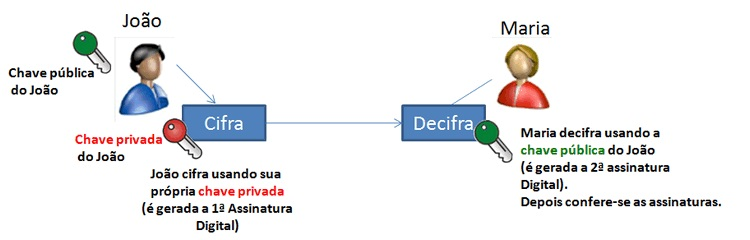
\includegraphics[width=\textwidth]{pics/chave_assimetrica_1}
		\caption{Criptografando com chaves assimétricas\footnote{Imagem extraída de: http://www.rtell.com.br}}
	\end{figure}
\end{frame}


%%% SLIDE %%%
\begin{frame}
\frametitle{Criptografia de Chaves Assimétricas}
\framesubtitle{Exemplos de Algoritmos}
\justifying Exemplos de algoritmos assimétricos populares:
	\begin{enumerate}
		\item {Protocolo Diffie-Hellman}
		\item {RSA (PKCS\#1)}
		\item {DSS (Digital Signature Standard), o qual incorpora o Algoritmo de Assinatura Digital}
		\item {ElGamal}
		\item {Criptosistema de Paillier}		
		\item {Criptosistema de Cramer–Shoup}
		\item {Protocolo de acordo de chave autenticada YAK}
		\item {Criptosistema NTRUEncrypt}
		\item {Criptosistema de McEliece}
	\end{enumerate}
\end{frame}

%%% SLIDE %%%
\begin{frame}
\frametitle{Criptografia de Chaves Assimétricas}
\framesubtitle{Exemplos de Protocolos}
\justifying Exemplos de protocolos que usam algoritmos de chaves assimétricas:
	\begin{enumerate}
		\item {S/MIME (Secure/Multipurpose Internet Mail Extension)\footnote{Em 14 de Maio de 2018, pesquisadores anunciaram o EFAIL. Vulnerabilidade nas tecnologias de criptografia de ponta a ponta OpenPGP e S/MIME que vazam o texto puro de e-mails criptografados.} }
		\item {PGP (Pretty Good Privacy)}
		\item {GPG/GnuPG (GNU Privacy Guard é uma alternativa GPL ao aplicativo PGP)}
		\item {ZRTP, um protocolo seguro VoIP}
		\item {SSL (Secure Socket Layer)}
		\item {TLS (Transport Layer Security)}
		\item {SSH (Secure Shell)}
		\item {Bitcoin} 
		\item {SILC (Secure Internet Live Conferencing)}
		\item {OTR (Off-the-Record Messaging)}	 
	\end{enumerate}
\end{frame}

%%% SLIDE %%%
\begin{frame}
\frametitle{Esquemas Híbridos}
A maioria dos protocolos de hoje são esquemas híbridos, ou seja, usam os dois esquemas:
	\begin{itemize}
		\item<+->{\textbf{Chaves Simétricas:} Usada, por exemplo, para encriptação e autenticação da mensagem.}
		\item<+->{\textbf{Chaves Assimétricas:} Usada, por exemplo, para a troca de chaves e assinatura digital.}
	\end{itemize}
\end{frame}

%%% SLIDE %%%
\begin{frame}
\frametitle{Assinatura Digital}
  \justifying É um método de autenticação de informação digital tipicamente tratada como substituta à assinatura física, já que elimina a necessidade de ter uma versão em papel do documento que necessita ser assinado.\\
  \textbf<+->{Propriedades da Assinatura Digital:}
  	\begin{itemize}
		\item<+->{\textbf{Autenticidade:} o receptor deve poder confirmar que a assinatura foi feita pelo emissor.}
		\item<+->{\textbf{Integridade:} qualquer alteração da mensagem faz com que a assinatura não corresponda mais ao documento.}
		\item<+->{\textbf{Irretratabilidade ou não-repúdio:} o emissor não pode negar a autenticidade da mensagem.}
	\end{itemize}
\end{frame}

%%% SLIDE %%%
\begin{frame}
\frametitle{Vamos para a Prática}
	\begin{figure}[h]
		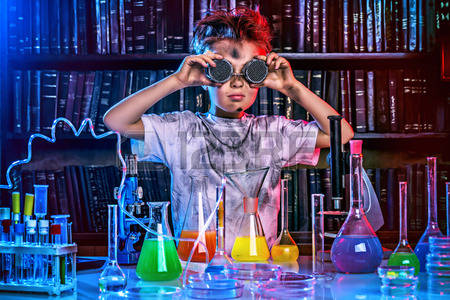
\includegraphics[width=\textwidth]{pics/pratica}
	\end{figure}
\end{frame}

%%% SLIDE %%%		
\begin{frame}
\frametitle{Ferramentas para usar no dia-a-dia (Linux e Windows)}
		\begin{enumerate}
			\item<+->{Assinatura de Arquivo}
			\item<+->{Criptografia de Arquivos}
			\item<+->{Assinatura de E-mail}
			\item<+->{Criptografia em E-mail}
			\item<+->{Chave GPG para Login em SSH}
		\end{enumerate}
\end{frame}

%%%% SLIDE %%%		
\begin{frame}
\frametitle{Lições Aprendidas}
\justifying
	\begin{enumerate}
		\item<+->{Nunca, jamais, desenvolva o seu próprio algoritmo de criptografia, a menos que você tenha uma equipe de experientes criptoanalistas verificando o seu projeto.}
		\item<+->{Não utilize algoritmos de criptografia não comprovados ou protocolos não comprovados.}
		\item<+->{Os atacantes vão sempre olhar para o ponto mais fraco de um sistema de criptografia. Por exemplo, um grande espaço de chaves por si só não é garantia de uma cifra segura; a cifra ainda pode estar vulnerável contra ataques analíticos.}
		\item<+->{Os algoritmos criptográficos podem ser fortes, mas as implementações sempre terão falhas. Mantenha seu software atualizado.}
	\end{enumerate}
\end{frame}

%%%% SLIDE %%%		
\begin{frame}
\frametitle{Lições Aprendidas}
\justifying
	\begin{enumerate}
		\setcounter{enumi}{4}
		\item<+->{Comprimentos de chave de algoritmos simétricos, a fim de frustrar ataques de busca exaustiva da chave:}
		\begin{itemize}
			\item<+->{64 bits: inseguro exceto para dados cujo uso se dará num prazo muito curto.}
			\item<+->{128 bits: segurança de longo prazo para várias décadas, a menos que os computadores quânticos se tornem disponíveis (computadores quânticos não existem e talvez nunca existam).}
			\item<+->{256 bits: como acima, mas provavelmente seguros até contra ataques por computadores quânticos.}
		\end{itemize}
	\end{enumerate}
\end{frame}

%%%% SLIDE %%%		
\begin{frame}{Considerações Finais}
\end{frame}

%%% BIBLIOGRAFIA %%%
%\begin{frame}[allowframebreaks]
	%%\usepackage[fixlanguage]{babelbib}
	%%\selectbiblanguage{brazil}
	%\frametitle{Referências}
	%\bibliographystyle{plain}
	%\bibliography{bibliografia}
%\end{frame}

\end{document}

